\documentclass[11pt, a4paper]{article}
\newcommand{\HomeworkHeader}{L02\_12-L02\_13}
% Shared LaTeX preamble for homework/*/main.tex

% --- Base layout ---
\usepackage[a4paper, top=2.5cm, bottom=2.5cm, left=2cm, right=2cm]{geometry}
\usepackage{fontspec}
\usepackage{xeCJK} % CJK fallback to avoid missing glyphs in Latin fonts
\usepackage{amsmath, amssymb, amsthm}
\usepackage{mathtools}
\usepackage{fancyhdr}
\usepackage{lastpage}
\usepackage[svgnames]{xcolor}
\usepackage{tikz}
\usetikzlibrary{automata, positioning, arrows.meta, bending, backgrounds}
\usepackage{pgfplots}
\pgfplotsset{compat=1.18}
\usepackage[most]{tcolorbox}
\usepackage{enumitem}

% --- Languages & fonts ---
\usepackage[english]{babel}
\babelprovide[import, main]{chinese}

\babelfont{rm}[UprightFont=*, BoldFont=* Bold, ItalicFont=* Italic, Scale=1.05]{Linux Libertine O}
\babelfont{sf}[UprightFont=*, BoldFont=* Bold, Scale=1.05]{Linux Biolinum O}
\babelfont[chinese]{rm}[
    UprightFont=*-Regular,
    BoldFont=*-Bold,
    ItalicFont=*-Regular,
    BoldItalicFont=*-Bold
]{Noto Serif CJK SC}
\babelfont[chinese]{sf}[
    UprightFont=*-Regular,
    BoldFont=*-Bold
]{Noto Sans CJK SC}
\babelfont{tt}{Noto Sans Mono}
\babelfont[chinese]{tt}{Noto Sans Mono CJK SC}

% xeCJK font setup (kept consistent with babelfont)
\setCJKmainfont{Noto Serif CJK SC}
\setCJKsansfont{Noto Sans CJK SC}
\setCJKmonofont{Noto Sans Mono CJK SC}

% --- Colors ---
\definecolor{primaryColor}{RGB}{46, 52, 64}
\definecolor{accentColor}{RGB}{94, 129, 172}
\definecolor{boxFill}{RGB}{236, 240, 241}
\definecolor{solLine}{RGB}{163, 190, 140}
\definecolor{expandColor}{RGB}{191, 97, 106}

% --- TikZ styles (DFA / NFA / PDA) ---
\tikzset{
    dfa_state/.style={
        state,
        thick,
        draw=accentColor,
        fill=boxFill,
        text=primaryColor,
        minimum size=1.1cm
    },
    dfa_edge/.style={
        ->,
        >=stealth,
        thick,
        draw=primaryColor,
        auto
    },
    pda_node/.style={
        state,
        thick,
        draw=accentColor,
        fill=boxFill,
        text=primaryColor,
        minimum size=1.2cm
    },
    pda_edge/.style={
        ->,
        >=stealth,
        thick,
        draw=primaryColor,
        auto
    },
    rule_expand/.style={
        pda_edge,
        draw=expandColor,
        text=expandColor
    },
    rule_match/.style={
        pda_edge,
        draw=solLine,
        text=solLine!80!black
    }
}

% --- Header / footer ---
\pagestyle{fancy}
\fancyhf{}
\lhead{\color{accentColor}\textbf{形式语言与自动机作业}}
\rhead{\color{primaryColor}\textbf{\HomeworkHeader}}
\cfoot{\small 第 \thepage \ 页,共 \pageref{LastPage} 页}
\setlength{\headheight}{24pt}
\addtolength{\topmargin}{-12pt}
\setlength{\emergencystretch}{2em}
\renewcommand{\headrulewidth}{0.4pt}
\renewcommand{\headrule}{\hbox to\headwidth{\color{accentColor}\leaders\hrule height \headrulewidth\hfill}}

% --- Problem box ---
\newtcolorbox[auto counter]{problem}[1][]{
    enhanced,
    breakable,
    colback=boxFill,
    colframe=accentColor,
    coltitle=white,
    fonttitle=\bfseries\large,
    title={题目 ~\thetcbcounter \quad #1},
    boxrule=0.5mm,
    arc=3mm,
    drop shadow=black!15!white,
    attach boxed title to top left={xshift=0.5cm, yshift*=-3mm},
    boxed title style={colback=accentColor}
}

% --- Solution environment ---
\newenvironment{solution}{
    \par\vspace{10pt}
    \noindent\textbf{\color{solLine} \Large \textit{Solution.}} \par
    \begingroup\color{primaryColor}\sloppy
    \leftskip1em \rightskip1em
    \noindent\rule{\textwidth}{0.4pt}
    \par\vspace{5pt}
}{
    \par\vspace{10pt}
    \noindent\rule[0.5ex]{\textwidth}{0.1pt}
    \endgroup
    \vspace{1.2cm}
}

% --- Title ---
\newcommand{\makeCustomTitle}[1]{
    \begin{center}
        \vspace*{1cm}
        {\Huge \bfseries \color{primaryColor} 作业 #1}\\
        \vspace{0.5cm}
        {\Large \color{accentColor} \today}
        \vspace{1.2cm}
    \end{center}
}


% Preamble shared in ../_shared/preamble.tex

\begin{document}

% 生成标题
\makeCustomTitle{L2.12 - L2.13:构造 PDA}

\section*{前言:构造方法说明}

本作业中所有题目均要求构造接受上下文无关文法(CFG)的下推自动机(PDA)。我们采用\textbf{空栈接受(Acceptance by Empty Stack)}的标准构造方法。

对于给定的 CFG $G = (V, \Sigma, R, S)$,构造 PDA
\[
M = (\{q\}, \Sigma, V \cup \Sigma, \delta, q, S, \emptyset),
\]
其中转换函数 $\delta$ 定义如下:
\begin{enumerate}
    \item \textbf{\textcolor{expandColor}{非终结符展开规则}}:对于每个产生式 $A \to \alpha \in R$,加入转换 $\delta(q, \epsilon, A) \ni (q, \alpha)$。
    \item \textbf{\textcolor{solLine!80!black}{终结符匹配规则}}:对于每个终结符 $a \in \Sigma$,加入转换 $\delta(q, a, a) = \{(q, \epsilon)\}$。
\end{enumerate}

\noindent\textit{注:在下方的状态图中,\textcolor{expandColor}{红色箭头}表示展开规则,\textcolor{solLine!80!black}{绿色箭头}表示匹配规则。}

\bigskip
\hrule
\bigskip

% --- 题目 1 ---
\begin{problem}
    构造 PDA 接受由文法 $S \rightarrow aSbb \mid aab$ 产生的语言。
\end{problem}

\begin{solution}
    \textbf{1. 构造转换函数 $\delta$}
    \begin{itemize}
        \item \textbf{\textcolor{expandColor}{Stack Operations (展开):}}
        \[
            \delta(q, \epsilon, S) = \{ (q, aSbb), (q, aab) \}
        \]
        \item \textbf{\textcolor{solLine!80!black}{Input Matching (匹配):}}
        \[
        \begin{aligned}
            \delta(q, a, a) &= \{(q, \epsilon)\},\\
            \delta(q, b, b) &= \{(q, \epsilon)\}
        \end{aligned}
        \]
    \end{itemize}

    \textbf{2. PDA 状态转移图}

    \begin{center}
    \begin{tikzpicture}[node distance=3cm]
        \node[pda_node, initial] (q) {$q$};

        \draw
        (q) edge [loop above, rule_expand]
            node [align=center] {$\epsilon, S \to aSbb$ \\ $\epsilon, S \to aab$} (q)
        (q) edge [loop right, rule_match]
            node [align=center] {$a, a \to \epsilon$ \\ $b, b \to \epsilon$} (q);
    \end{tikzpicture}
    \end{center}

    \textbf{3. 分析}

    该 PDA 只有一个状态 $q$。开始时栈内放入 $S$。如果栈顶是 $S$,PDA 猜测并将其替换为 $aSbb$ 或 $aab$;如果栈顶是终结符且与输入符号一致,则消去栈顶符号。栈最终为空时接受。
\end{solution}

% --- 题目 2 ---
\begin{problem}
    构造 PDA 接受由文法 $S \rightarrow aSSS \mid ab$ 产生的语言。
\end{problem}

\begin{solution}
    \textbf{1. 构造转换函数 $\delta$}
    \begin{itemize}
        \item \textbf{\textcolor{expandColor}{展开规则:}}
        \[
            \delta(q, \epsilon, S) = \{ (q, aSSS), (q, ab) \}
        \]
        \item \textbf{\textcolor{solLine!80!black}{匹配规则:}}
        \[
        \begin{aligned}
            \delta(q, a, a) &= \{ (q, \epsilon) \},\\
            \delta(q, b, b) &= \{ (q, \epsilon) \}
        \end{aligned}
        \]
    \end{itemize}

    \textbf{2. PDA 状态转移图}

    \begin{center}
    \begin{tikzpicture}[node distance=3cm]
        \node[pda_node, initial] (q) {$q$};

        \draw
        (q) edge [loop above, rule_expand, looseness=8]
            node [align=center] {$\epsilon, S \to aSSS$ \\ $\epsilon, S \to ab$} (q)
        (q) edge [loop right, rule_match, looseness=8]
            node [align=center] {$a, a \to \epsilon$ \\ $b, b \to \epsilon$} (q);
    \end{tikzpicture}
    \end{center}
\end{solution}

% --- 题目 3 ---
\begin{problem}[多非终结符文法]
    构造对应如下文法的 PDA:
    \[
    \begin{aligned}
    S &\rightarrow aABB \mid aAA \\
    A &\rightarrow aBB \mid a \\
    B &\rightarrow bBB \mid A
    \end{aligned}
    \]
\end{problem}

\begin{solution}
    \textbf{1. 转换函数 $\delta$ 详解}

    \begin{itemize}
        \item $S$ 的展开:\textcolor{expandColor}{$\delta(q, \epsilon, S) = \{ (q, aABB), (q, aAA) \}$}
        \item $A$ 的展开:\textcolor{expandColor}{$\delta(q, \epsilon, A) = \{ (q, aBB), (q, a) \}$}
        \item $B$ 的展开:\textcolor{expandColor}{$\delta(q, \epsilon, B) = \{ (q, bBB), (q, A) \}$}
        \item 终结符匹配:\textcolor{solLine!80!black}{$\delta(q, a, a) = \{ (q, \epsilon) \}$;\\
        \textcolor{solLine!80!black}{$\delta(q, b, b) = \{ (q, \epsilon) \}$}}
    \end{itemize}

    \textbf{2. PDA 状态转移图}

    \begin{center}
    \begin{tikzpicture}[node distance=4cm]
        \node[pda_node, initial] (q) {$q$};

        % Self-loops 分散到不同方向,避免文字重叠
        \draw
        (q) edge [loop above, rule_expand, in=120, out=60, looseness=4]
            node [align=center, yshift=5mm]
                {$\epsilon, S \to aABB$ \\ $\epsilon, S \to aAA$} (q)
        (q) edge [loop left, rule_expand, in=210, out=240, looseness=8]
            node [align=center, xshift=-8mm, yshift=-1mm]
                {$\epsilon, A \to aBB \mid a$ \\ $\epsilon, B \to bBB \mid A$} (q)
        (q) edge [loop below, rule_match, in=-120, out=-60, looseness=6]
            node [align=center, yshift=-5mm]
                {$a, a \to \epsilon$ \\ $b, b \to \epsilon$} (q);
    \end{tikzpicture}
    \end{center}

    \textit{图注:为了保持整洁,部分相同左部的规则合并显示。}
\end{solution}

% --- 题目 4 ---
\begin{problem}[相互递归文法]
    构造 PDA 接受由如下文法产生的语言:
    \[
        S \rightarrow AA \mid a, \quad A \rightarrow SA \mid b
    \]
\end{problem}

\begin{solution}
    \textbf{1. 转换函数 $\delta$ 表}

    \begin{center}
    % 使用 tcolorbox 包装表格
    \begin{tcolorbox}[colback=white, colframe=primaryColor, width=0.9\textwidth, arc=2mm]
    \centering
    \begin{tabular}{c c c l}
    \textbf{\color{primaryColor}类型} & \textbf{输入} & \textbf{栈顶} & \textbf{动作 (栈变化)} \\
    \hline
    \textcolor{expandColor}{展开} & $\epsilon$ & $S$ & $\to AA$ \\
    \textcolor{expandColor}{展开} & $\epsilon$ & $S$ & $\to a$ \\
    \textcolor{expandColor}{展开} & $\epsilon$ & $A$ & $\to SA$ \\
    \textcolor{expandColor}{展开} & $\epsilon$ & $A$ & $\to b$ \\
    \hline
    \textcolor{solLine!80!black}{匹配} & $a$ & $a$ & $\to \epsilon$ (pop) \\
    \textcolor{solLine!80!black}{匹配} & $b$ & $b$ & $\to \epsilon$ (pop) \\
    \end{tabular}
    \end{tcolorbox}
    \end{center}

    \textbf{2. PDA 状态转移图}

    \begin{center}
    \begin{tikzpicture}[node distance=3cm]
        \node[pda_node, initial] (q) {$q$};

        \draw
        (q) edge [loop above, rule_expand, looseness=8]
            node [align=center]
                {$\epsilon, S \to AA \mid a$ \\ $\epsilon, A \to SA \mid b$} (q)
        (q) edge [loop right, rule_match, looseness=8]
            node [align=center]
                {$a, a \to \epsilon$ \\ $b, b \to \epsilon$} (q);
    \end{tikzpicture}
    \end{center}

    此图展示了 PDA 如何在单状态 $q$ 下,通过非确定性选择(红色路径)不断重写栈顶符号,或者通过匹配(绿色路径)消去终结符。当输入读完且栈为空时接受。
\end{solution}

\end{document}
